\documentclass{article}
\usepackage{tikz}
\usetikzlibrary{arrows.meta,positioning,calc,shapes.geometric}
\pagestyle{empty}
\begin{document}
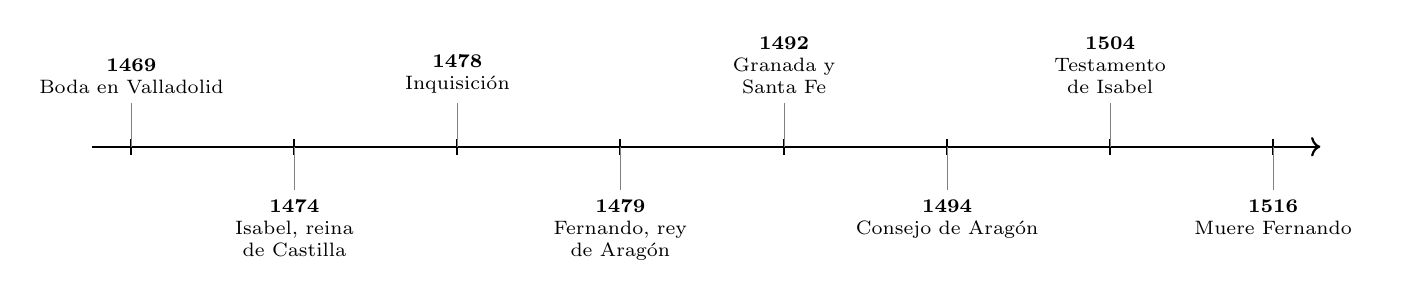
\begin{tikzpicture}
\tikzset{every node/.append style={align=center}}
\draw[->, thick] (-0.5,0) -- (15.10,0);
\draw[thick] (0.00,-0.1) -- (0.00,0.1);
\draw[gray] (0.00,0) -- (0.00,0.55);
\node[anchor=south, align=center, text width=2.40cm, font=\scriptsize] at (0.00,0.55) {\textbf{1469}\\ Boda en Valladolid};
\draw[thick] (2.07,-0.1) -- (2.07,0.1);
\draw[gray] (2.07,0) -- (2.07,-0.55);
\node[anchor=north, align=center, text width=2.40cm, font=\scriptsize] at (2.07,-0.55) {\textbf{1474}\\ Isabel, reina de Castilla};
\draw[thick] (4.14,-0.1) -- (4.14,0.1);
\draw[gray] (4.14,0) -- (4.14,0.55);
\node[anchor=south, align=center, text width=2.40cm, font=\scriptsize] at (4.14,0.55) {\textbf{1478}\\ Inquisición};
\draw[thick] (6.21,-0.1) -- (6.21,0.1);
\draw[gray] (6.21,0) -- (6.21,-0.55);
\node[anchor=north, align=center, text width=2.40cm, font=\scriptsize] at (6.21,-0.55) {\textbf{1479}\\ Fernando, rey de Aragón};
\draw[thick] (8.29,-0.1) -- (8.29,0.1);
\draw[gray] (8.29,0) -- (8.29,0.55);
\node[anchor=south, align=center, text width=2.40cm, font=\scriptsize] at (8.29,0.55) {\textbf{1492}\\ Granada y Santa Fe};
\draw[thick] (10.36,-0.1) -- (10.36,0.1);
\draw[gray] (10.36,0) -- (10.36,-0.55);
\node[anchor=north, align=center, text width=2.40cm, font=\scriptsize] at (10.36,-0.55) {\textbf{1494}\\ Consejo de Aragón};
\draw[thick] (12.43,-0.1) -- (12.43,0.1);
\draw[gray] (12.43,0) -- (12.43,0.55);
\node[anchor=south, align=center, text width=2.40cm, font=\scriptsize] at (12.43,0.55) {\textbf{1504}\\ Testamento de Isabel};
\draw[thick] (14.50,-0.1) -- (14.50,0.1);
\draw[gray] (14.50,0) -- (14.50,-0.55);
\node[anchor=north, align=center, text width=2.40cm, font=\scriptsize] at (14.50,-0.55) {\textbf{1516}\\ Muere Fernando};
\end{tikzpicture}
\end{document}
